%\section{Vizuelizacija}
%\label{sec:Vizuelizacija}

Vizuelizacija originalnog skupa podataka je prikazana na slici \ref{fig:before}. Nedostaju\'c{}e vrednosti su prikazane belom bojom, dok su plavom bojom predstavljene postoju\'c{}e vrednosti atributa.

\begin{figure}[H]
    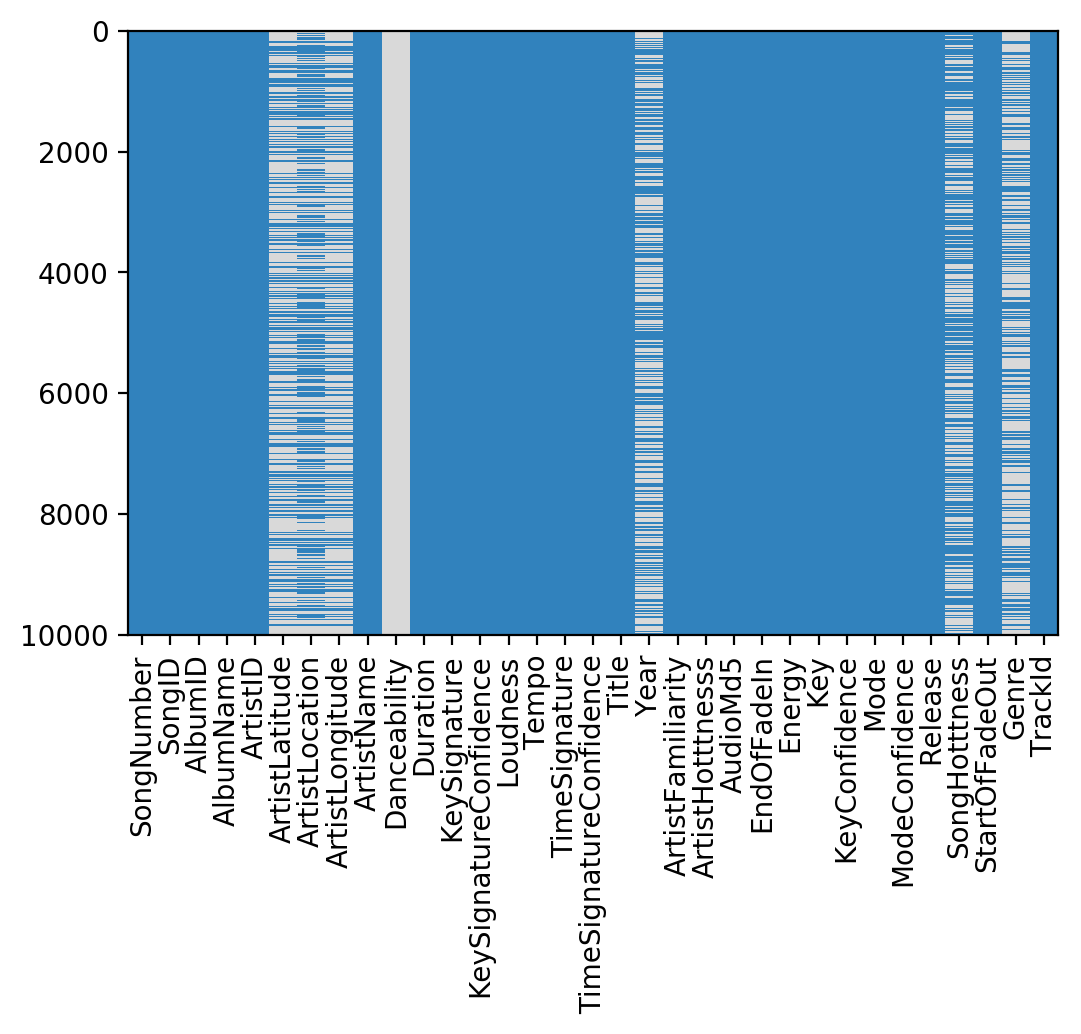
\includegraphics[scale=0.8]{resources/before_processing.png}
    \caption{Nedostaju\'c{}e vrednosti u originalnom skupu podataka}
    \label{fig:before}
\end{figure}

 Sa prikaza skupa podataka se vidi da atribut koji opisuje plesnu mo\'c{} pesme \emph{eng. dancability}, ni u jednom slu\v{c}aju nema postavljenu vrednost, te da je on neupotrebljiv. Takodje, godina, lokacija autora, geografska \v{s}irina, geografska du\v{z}ina i \v{z}anr su atributi koji u velikom broju slu\v{c}ajeva nemaju vrednost. Medjutim, zbog njihove va\v{z}nosti, mi \'c{}emo svoje istra\v{z}ivanje vr\v{s}iti nad onim slogovima za koje su ove vrednosti poznate. Nakon izdvajanja relevantnih atributa za na\v{s}e istra\v{z}ivanje, pripremljen skup podataka je prikazan na slici \ref{fig:after}.

\begin{figure}[H]
    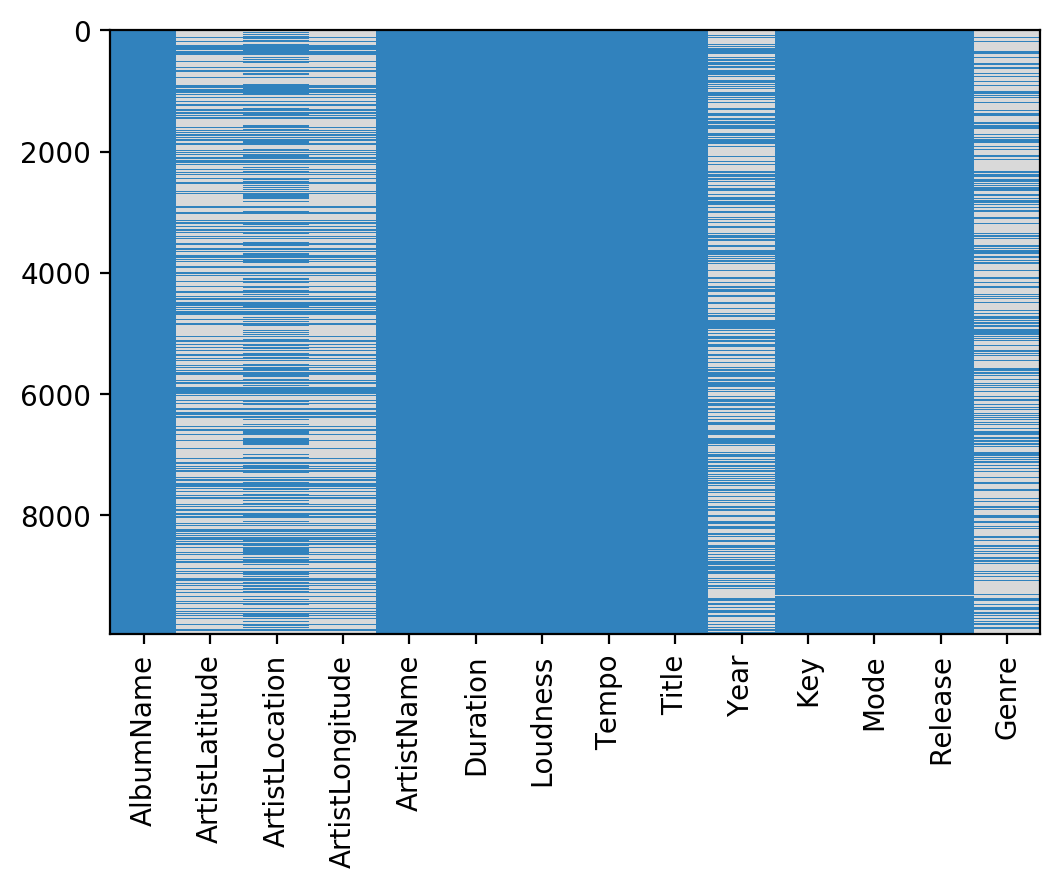
\includegraphics[scale=0.8]{resources/after_processing.png}
    \caption{Izdvojeni atributi kori\v{s}\'c{}eni u istra\v{z}ivanju}
    \label{fig:after}
\end{figure}


Geografska rasprostranjenost autora \v{c}ije su se pesme na\v{s}le u skupu podataka se mo\v{z}e videti na slici \ref{fig:Geolokacija}. Razli\v{c}ite boje predstavljaju vizuelizaciju godine izdavanja pesme - gradijentni prelaz od plave (1950) do crvene (2010).

\begin{figure}[H]
    \centering
    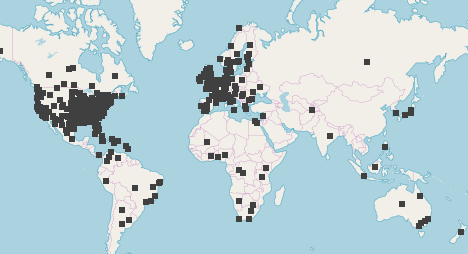
\includegraphics[scale=0.45]{resources/Geolokacija.png}
    \caption{Geografska rasprostranjenost autora}
    \label{fig:Geolokacija}
\end{figure}

Spisak najzastupljenijih zanrova u skupu se mo\v{z}e videti na slici \ref{fig:ZastupljenostZanrova}. \v{Z}anr je atribut sa velikom stopom nedostaju\'c{}ih vrednosti, uz dodatni problem re\v{c}enica prisutnih u nizu (podse\'c{}amo na problem naveden prilikom preprocesiranja, poglavlje \ref{sec:Preprocesiranje}), tako da je analiza vr\v{s}ena nad veoma ograni\v{c}enim skupom od oko tri hiljade slogova. Smatramo, da su ovi rezultati u velikoj meri sli\v{c}ni rezultatima koji bi se dobili da je potpuni skup analiziran - ukoliko ne bi bilo nedostaju\'c{}ih vrednosti za atribut \v{z}anr.

\begin{figure}[H]
    \centering
    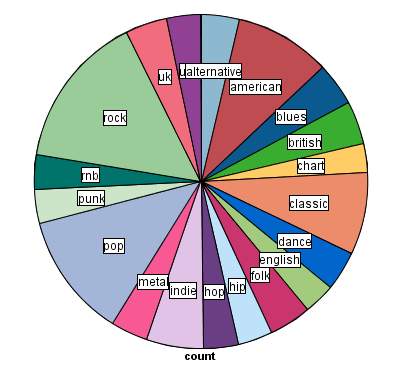
\includegraphics[scale=0.5]{resources/ZastupljenostZanrova.png}
    \caption{Zastupljenost \v{z}anrova}
    \label{fig:ZastupljenostZanrova}
\end{figure}

Vrednosti atributa \emph{duration} prikazane su na grafiku \ref{fig:duration}. Postoji jedna pesma koja ima negativnu du\v{z}inu pa smo najpre izbacili ovu pesmu iz skupa koji obradjujemo. Kako postoje izuzetno duge pesme, nismo postavili gornje ograni\v{c}enje za trajanje pesme.

\begin{figure}[H]
    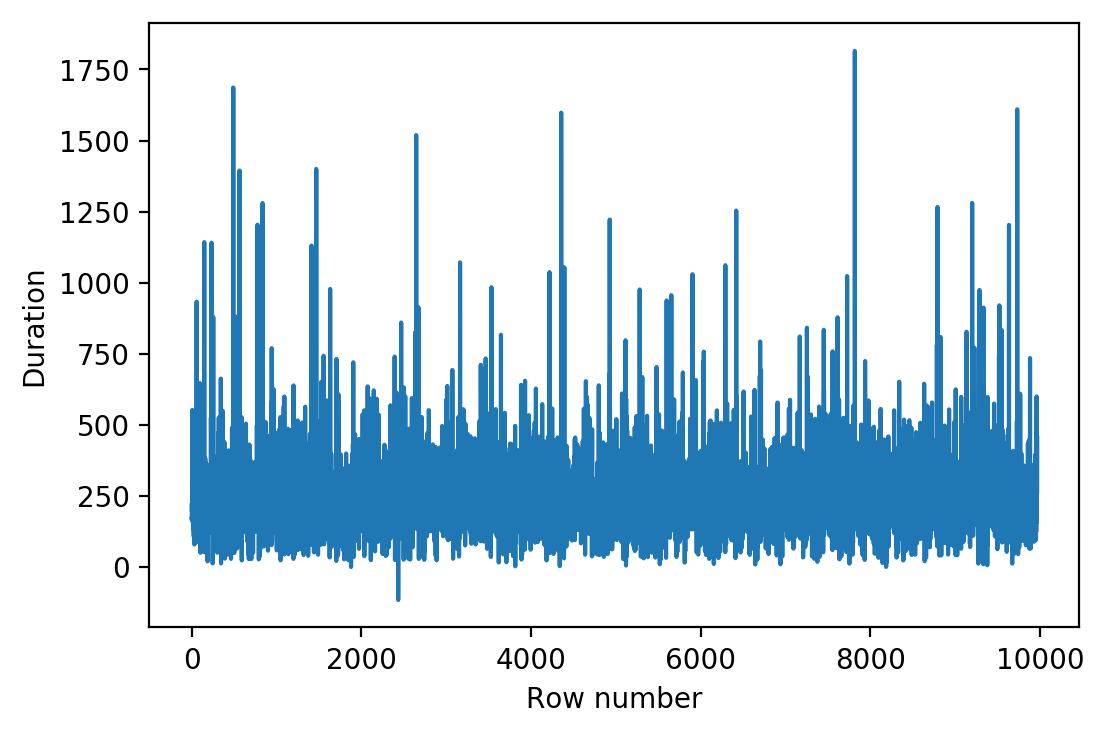
\includegraphics[scale=0.6]{resources/duration.png}
    \caption{Vrednosti atributa \emph{duration}}
    \label{fig:duration}
\end{figure}

Grafik zavisnosti godine i trajanja pesme se mo\v{z}e videti na slici \ref{fig:YearDuration}. Jedan zanimljiv zaklju\v{c}ak koji se name\'c{}e, je da se prose\v{c}no trajanje pesama pove\'c{}ava kroz vreme, sa razlikom od oko 20 sekundi u odnosu na 50-te godine pro\v{s}log veka. Detaljniji prikaz promene proseka trajanja se mo\v{z}e videti na slici \ref{fig:YearDurationAvg}. Takodje, jasno je da se i raznovrsnost pesama mnogo ve\'c{}a danas - prisutne su i veoma kratke ali i veoma duga\v{c}ke pesme.


\begin{figure}[H]
    \centering
    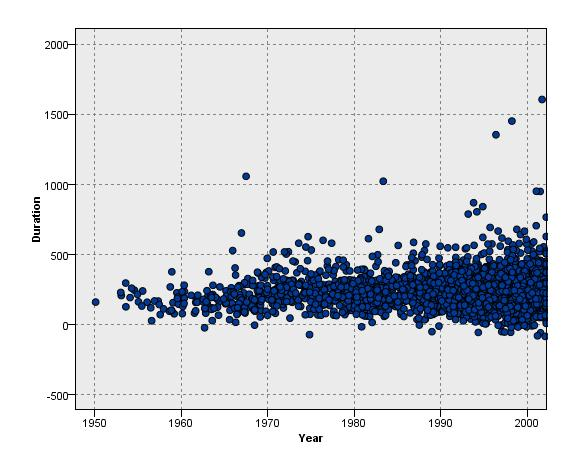
\includegraphics[scale=0.52]{resources/year-duration.jpg}
    \caption{Odnos godine izdavanja i du\v{z}ine pesme}
    \label{fig:YearDuration}
\end{figure}

\begin{figure}[H]
    \centering
    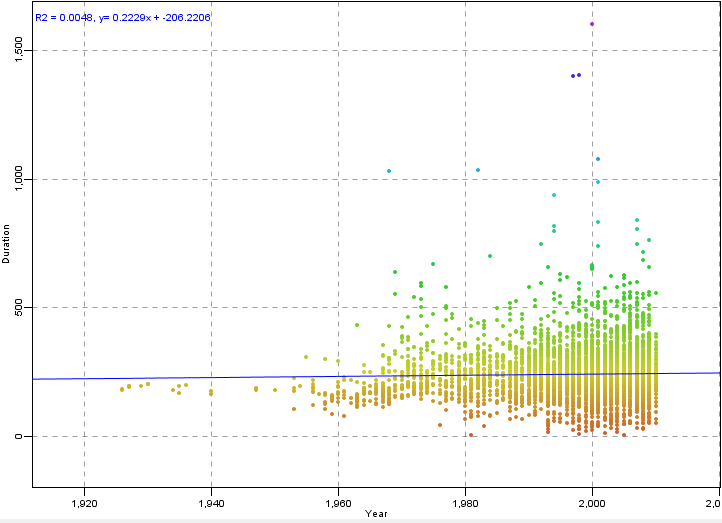
\includegraphics[scale=0.5]{resources/year-duration.PNG}
    \caption{Promena proseka du\v{z}ine pesama kroz vreme}
    \label{fig:YearDurationAvg}
\end{figure}


Prose\v{c}na du\v{z}ina pesama po dr\v{z}avama je prikazana na slici \ref{fig:CountryDuration}. Na\v{z}alost, nisu svi slogovi imali informaciju o nazivu dr\v{z}ave. Iz ovog razloga, dobijenim rezultatima ne treba pridavati veliki zna\v{c}aj.

\begin{figure}[H]
    \centering
    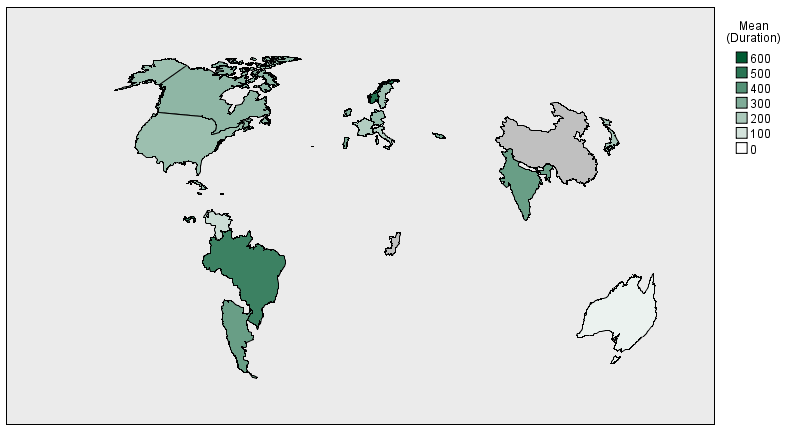
\includegraphics[scale=0.45]{resources/country-duration.png}
    \caption{Prose\v{c}na du\v{z}ina pesama na raznim lokacijama}
    \label{fig:CountryDuration}
\end{figure}


Na slici \ref{fig:loudness} prikazane su vrednosti atributa \emph{loudness}. Ove vrednosti su dobijene na osnovu njihovih proseka tokom trajanja pesme, kao i nekim dodatnim transformacijama. Vise o ovome se mo\v{z}e na\'c{} na zvani\v{c}nom sajtu skupa \cite{Dataset}. Sa grafika se vidi da za atribut \emph{loudness} postoje vrednosti koje izuzetno odstupaju od proseka. Iz toga razloga smo prilikom istra\v{z}ivanja koristili pesme sa vredno\v{s}\'c{}u atributa iz skupa $[-40, 0]$.

\begin{figure}[H]
    \centering
    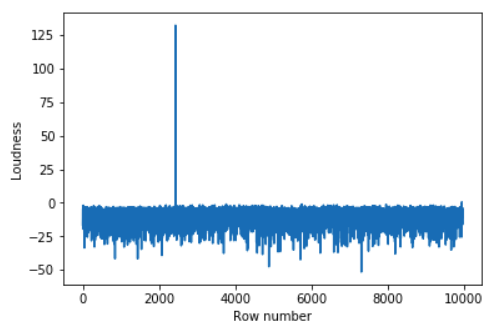
\includegraphics[scale=0.55]{resources/loudness.png}
    \caption{Vrednosti atributa \emph{loudness}}
    \label{fig:loudness}
\end{figure}

Na slici \ref{fig:tempo} prikazane su vrednosti atributa \emph{tempo}. Ovaj atribut sadr\v{z}i nekoliko vrednosti koje su dosta ispod proseka. Medjutim, postoji verovatno\'c{}a da su njima predstvaljene nadprose\v{c}no spore pesme te zbog toga nismo vr\v{s}ili nikakvo odsecanje.

\begin{figure}[H]
    \centering
    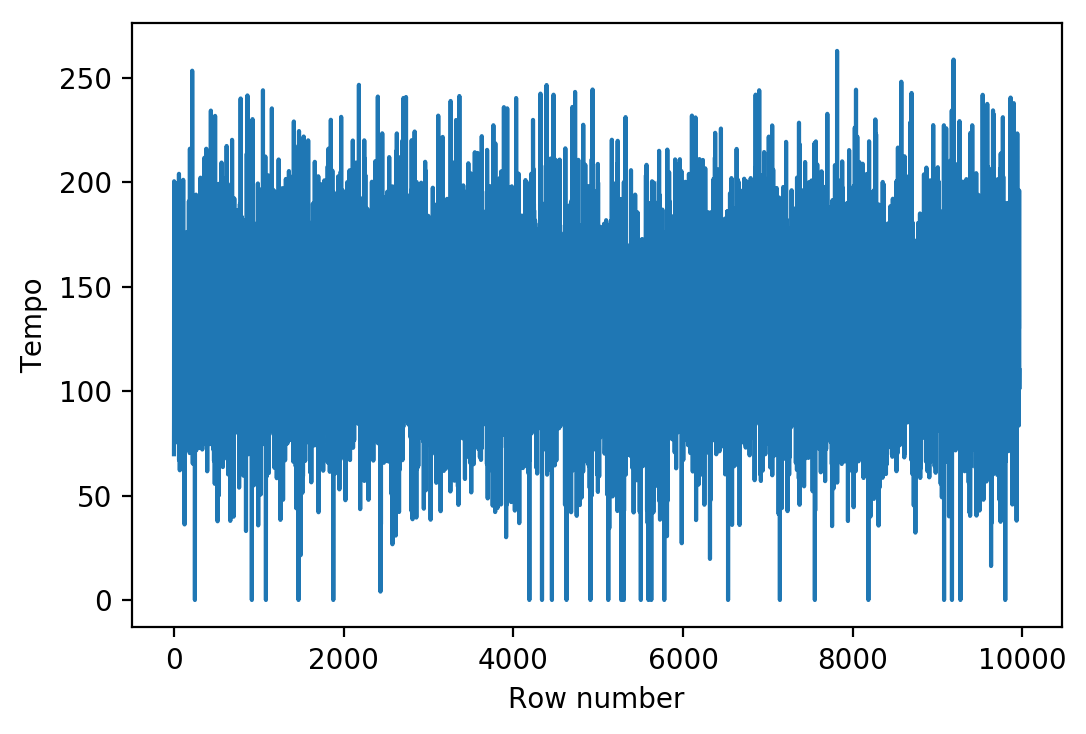
\includegraphics[scale=0.6]{resources/tempo.png}
    \caption{Vrednosti atributa \emph{tempo}}
    \label{fig:tempo}
\end{figure}

S obzirom da \'c{}emo atribute \emph{loudness}, \emph{tempo} i \emph{mode} \footnote{loudness, tempo i mode predstavljaju prose\v{c}nu ja\v{c}inu, tempo i mod (dur ili mol), redom.} koristiti u daljoj analizi (predikcija \v{z}anra pesme) u poglavlju \ref{sec:Klasifikacija}, prikaza\'c{}emo i grafi\v{c}ki prikaz njihove zavisnosti na slici \ref{fig:TempoMode}. Mo\v{z}e se videti da iako pesme oba moda uzimaju raznolike vrednosti za tempo i ja\v{c}inu, mogu\'c{}e je uo\v{c}iti da se pesme sa ekstremnim vrednostima za tempo lep\v{s}e dele po modu. Takodje, mnogo tihe pesme obi\v{c}no pripadaju jednom modu, \v{s}to je i za o\v{c}ekivati jer molske pesme su nekada jako tihe.

\begin{figure}[H]
    \centering
    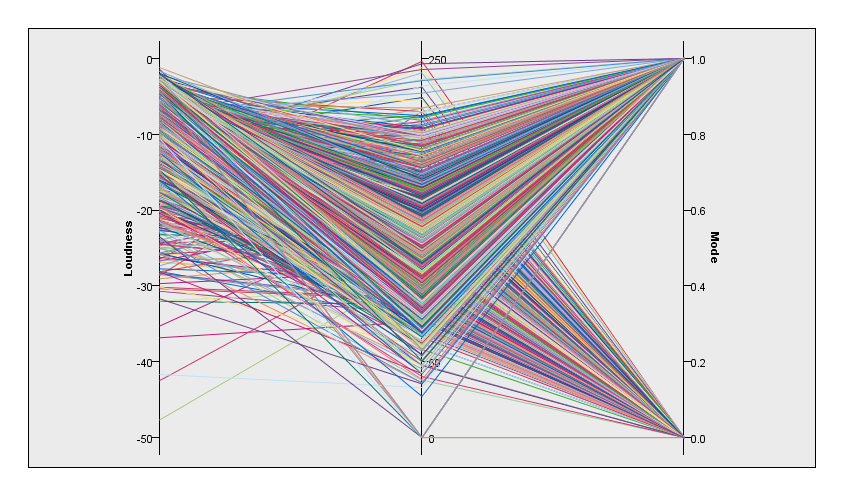
\includegraphics[scale=0.4]{resources/tempo-loudness-mode.png}
    \caption{Prikaz tempa, ja\v{c}ine i moda (dur ili mol)}
    \label{fig:TempoMode}
\end{figure}
